\section{Background and Related Work}

\subsection{Stable Matching Problem}\label{ss:smp}
In this study, we evaluate our model with a typical two-sided problem of stable matching.
An instance $I$ of a stable matching problem consists of two sets of agents $A$ and $B$ on a bipartite graph. 
Fig.~\ref{fig:stable_matching} illustrates an example of $I$. 
Each agent $a_i$ in $A~(0<i\leq N)$ has a preference list $p^A_i$, which is an ordered set of elements in $B$ and $p^A_{ij}=rank(b_j;p^A_i)$ is the index of $b_j$ in the list $p^A_i$.
$a_i$ prefers $b_j$ to $b_{j'}$ if $p^A_{ij}<p^A_{ij'}$.
Similarly, each agent $b_j$ in $B (0<j\leq M)$ has a preference list $p_j^B$.


\begin{figure}[ht!]
    \centering
    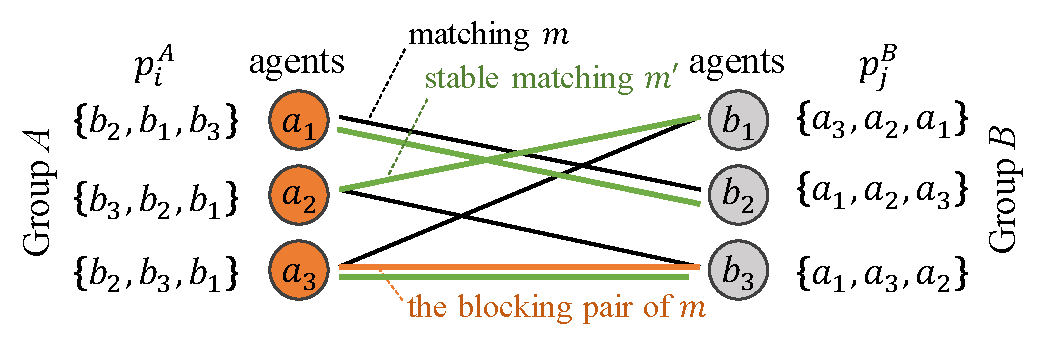
\includegraphics[width=1.0\linewidth]{figures/stable_matching.pdf}
    \caption{
    An example of a stable matching instance with a size of $N=3$. The matching $m$ (black edges) is not stable due to the blocking pair (the orange edge). The matching $m'$ (green edges) is a stable matching.}
    %\vspace{-0.5em}
    %\jm{I think $p_i, p_j$ should all be written as $p^A_i, p^B_j$.}\ah{could you revise it?}
    \label{fig:stable_matching}
\end{figure}


%Consider a bipartite graph $K_{N,M}=G(A, B, E)$, where $E=A\times B$. 
%A matching $m$ is a subset of $E$ whose edges do not share any nodes (see the black edges in Fig.~\ref{fig:stable_matching} for an example).

For a matching $m \in \{0,1\}^{N\times M}$, we say that an unmatched pair $\{a_v, b_w\}(\notin m)$ blocks $m$ if there are matched pairs $\{a_v,b_j\}\in m$ and $\{a_i,b_w\}\in m$ that satisfy $p^A_{vw} < p^A_{vj}$ and $p^B_{wv} < p^B_{wi}$. Here, $\{a_v, b_w\}$ is called a blocking pair (the orange edge blocks a matching of black edges in the figure).

A matching is called stable if it has no blocking pair (the green edges in the figure).
It is known that an instance $I$ always has at least one stable matching, and the Gale-Shapley (GS) algorithm can find it in $O(N^2)$ \cite{gale1962college}.
%\footnote{Also known as the Deferred Acceptance (DA) algorithm} 
%\jm{I suggest the footnote here is unnecessary.}\ah{removed.}
%In the GS algorithm, agents in one side propose to the other side iteratively in an order of preference. As a result, the stable matching obtained by the GS algorithm is always most biased where the proposer side can get the most preferable result while the recipient side only gets the least preferable result among all the possibilities of stable matching.
However, the algorithm prioritizes either side and the other side only gets the least preferable result among all the possibilities of stable matching.

\begin{table}[ht]
   \small
   \setlength\tabcolsep{4.0pt} % セルの左右の余白
    \centering
    \begin{tabular}{lrcl}
        \toprule
        \multicolumn{1}{c}{Cost} & \multicolumn{3}{c}{Definition} \\
        \midrule
        Sex equality  &  $\SEq(m;I)$ & $\!=\!$  & $|P(m;A)-P(m;B)|$ \\
        Regret        &  $Reg(m;I)$ & $\!=\!$  & $\max_{\{a_i,b_j\}\in m}(\max(p^A_{ij},p^B_{ji}))$ \\
        Egalitarian   &  $Egal(m;I)$& $\!=\!$  & $P(m;A)+P(m;B) $ \\
        Balance       &  $Bal(m;I)$ & $\!=\!$  & $\max(P(m;A),P(m;B)) $  \\   \bottomrule
    \end{tabular}
    %\vspace{-0.5em}
    \caption{Representative costs to measure the fairness of matching.}
    \label{tab:costs}
\end{table}

%\paragraph{Measures of Fairness}

To compensate for the unfairness, there have been diverse measures of fairness proposed, with different complexities of finding an optimal solution. They are listed in Table \ref{tab:costs} with the definitions, where
\begin{align}
    P(m;A) =\!\! \sum_{\{a_i,b_j\}\in m}\!\! p^A_{ij}, && P(m;B) =\!\! \sum_{\{a_i,b_j\}\in m}\!\! p^B_{ji}.  \label{eq:pref} 
\end{align}
\textbf{Sex equality cost} ($\SEq$) is a popular measure that focuses on the unfairness brought by the gap between the two sides' satisfaction \cite{gusfield1989stable}. 
\textbf{Regret cost} ($Reg$) measures the unfairness brought by the agent who obtained the least satisfaction (the weakest individual) in the matching.
\textbf{Egalitarian cost} ($Egal$) measures the overall satisfaction, in other words, the greater good, rather than concerning the weaker individual or weaker side \cite{gusfield1989stable}.
\textbf{Balance cost} ($Bal$) is a compromise between side-equality and overall satisfaction \cite{feder1995stable,gupta2019balanced}, and equivalent to $\frac{1}{2}(\SEq+Egal)$. 
Minimizing balance cost is to benefit the weaker side while less harming the stronger side. 

Among these measures, a stable matching of minimum regret cost and minimum egalitarian cost can be found in $O(N^2)$ and $O(N^3)$, respectively \cite{gusfield1987three,irving1987efficient,feder1992new}, while minimizing sex equality cost or balance cost is known as strongly NP-hard \cite{kato1993complexity,mcdermid2014sex,feder1995stable}.

There are several approximation solvers for the strongly NP-hard stable matching variants. Iwama \emph{et~al$.$} proposed a method that runs in $O(N^{3+\frac{1}{\varepsilon}})$ whose gap from the optimal solution is bounded by $\varepsilon$ \cite{iwama}.
Deferred Acceptance with Compensation Chains 
(\textit{DACC}) is an extension of the GS algorithm without prioritizing any side. 
It can terminate in $O(N^4)$ \cite{dworczak2016deferred}. 
\textit{PowerBalance} is a state-of-the-art algorithm.
In each round of proposing, it balances the two sides by letting the stronger side propose (because their satisfactions decrease if getting rejected). 
It was reported that PowerBalance has competitive performance when enforcing a termination in $O(N^2)$ \cite{tziavelis2019equitable}.

\subsection{Learning-based Matching Solvers}\label{ss:mlap}
Although learning-based matching solvers are still in the process of development, it has potential applications when we can only observe incomplete information.
The dynamic matching problem \cite{wang2019adaptive} is one typical case.
%, where agents can arrive and leave dynamically at any time (e.g., online MOT with occlusions). %Learning-based methods can deal with such task-dependent uncertainty without manually exploring the best-fit algorithm.
%\jm{do you mean ``Learning-based methods can deal with such uncertainty without manually designing a proper algorithm''?}\ah{What is the problem of the original sentence? IMO, ``proper'' is too vague to use in a pape. I've changed data-driven to task-dependent.}
%\jm{``task-dependent'' is good. Besides, I think the word ``taken into consideration'' is vague, and the word ``tailor'' is not usually seen for this kind of scene.}\ah{how about this?}
%Another case is temporal scene alignment between videos, where the optimal scene similarity measure is unknown, and we often design a feature encoder to solve this type of problem.
Another case is temporal alignment, where we have only superficial observation (videos, audio, or narration) and cannot access the true similarity between temporal events. Learning-based solvers would be helpful to jointly train the feature encoder with the matching module \cite{fathony2018efficient}.

Learning-based solvers also have advantages in flexibility even to deal with variations of traditional matching problems (e.g., incomplete preference lists with ties, continuous preference scores, or multi-dimensional preference \cite{multi_stable_matching}) as well as more complex objective functions (e.g., a weighted sum of costs in Table \ref{tab:costs}).
Aiming to develop learning-based methods for the stable matching problem, \cite{harvard2019} proposed a loss function that relaxes the discrete constraints on matching stability into a continuous measure, which enables to train a model in an unsupervised manner.
However, they only provide an experiment on $N=5$ with a shallow neural network.

Deep Bipartite Matching (DBM) \cite{gibbons2019deep} is another attempt to approximate the (not strongly) NP-hard problem of weapon-target assignment (WTA), but its performance is not at a comparative level with the state-of-the-art of WTA approximation
\cite{ahuja2007exact} even limiting the size of problem instances.
